\subsubsection{Akurasi Segmentasi InternImage}
\label{sec:akurasi_segmentasi}

Model InternImage dengan backbone DCNv3~\parencite{wang2023internimage} dilatih pada dataset lokal kampus ITS melalui \emph{fine-tuning} dari bobot pralatih Mapillary Vistas.
Proses pelatihan dilakukan selama 50 epoch menggunakan \emph{loss function Cross-Entropy}.
Kurva pelatihan dan validasi disajikan pada Gambar~\ref{fig:training_curve}.

\begin{figure}[H]
    \centering
    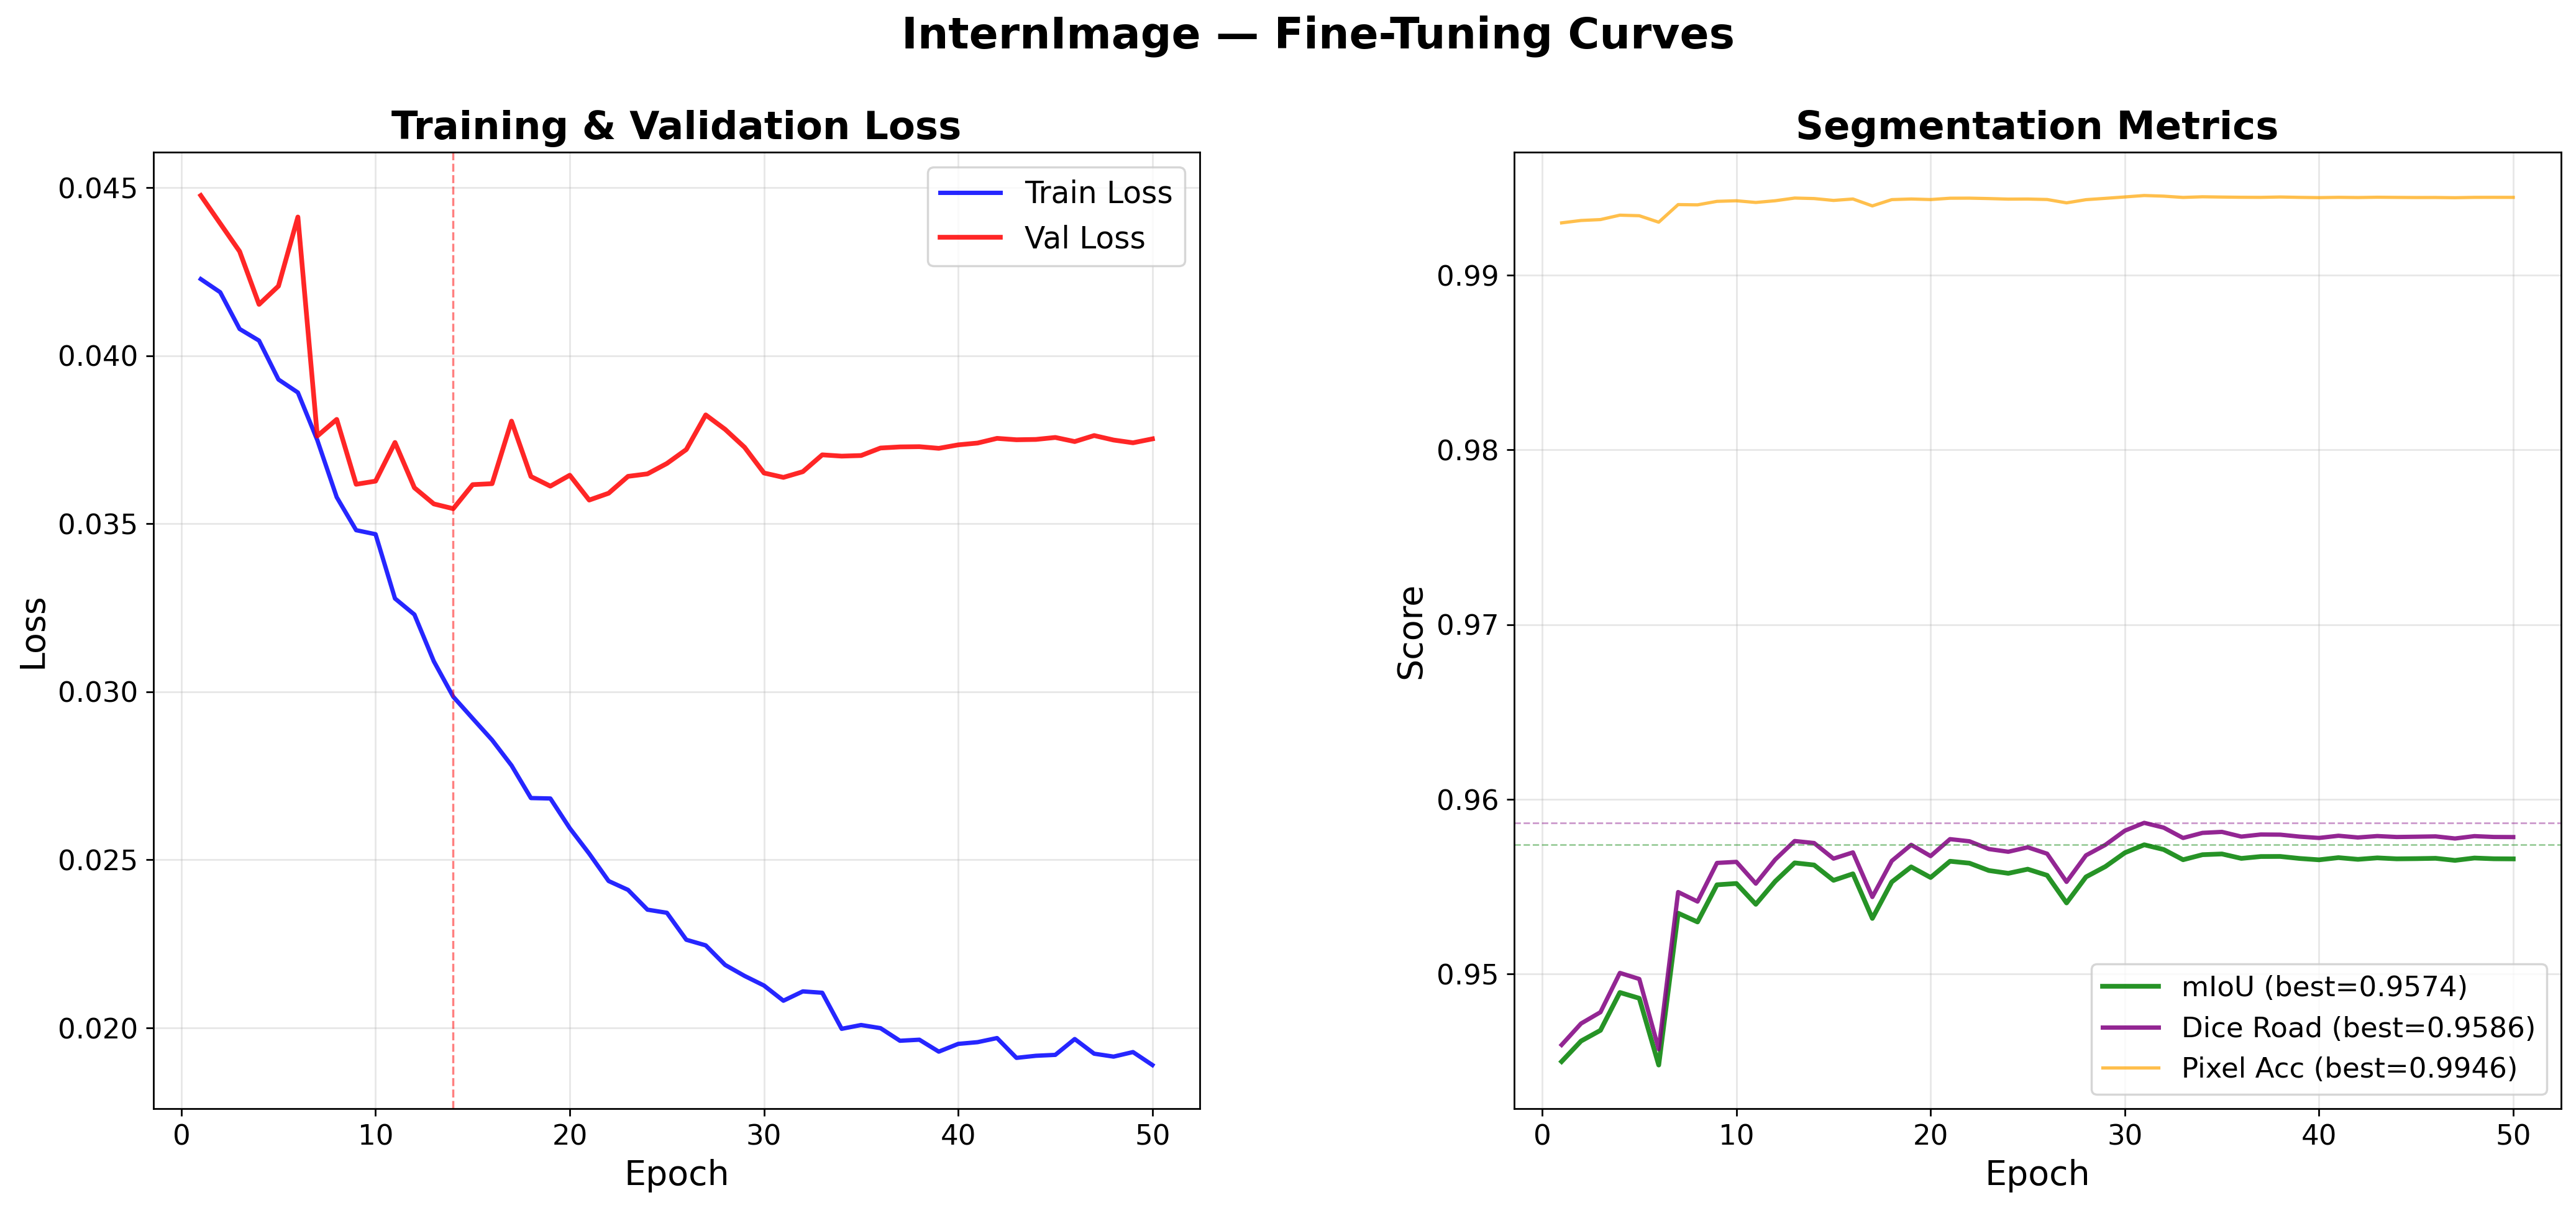
\includegraphics[width=1.0\textwidth]{gambar/training_curve.png}
    \caption{Kurva pelatihan model InternImage selama 50 epoch dan metrik segmentasi}
    \label{fig:training_curve}
\end{figure}

Model konvergen pada epoch ke-14 dengan \emph{validation loss} sebesar 0,0354.
Performa terbaik dicapai pada epoch ke-31 dengan metrik yang ditampilkan Tabel~\ref{tab:metrik_segmentasi}.

\begin{table}[H]
\centering
\caption{Hasil pelatihan model InternImage pada dataset lokal ITS}
\label{tab:metrik_segmentasi}
\begin{tabular}{l c}
\hline
\textbf{Metrik} & \textbf{Nilai} \\
\hline
mIoU            & 0,9574 \\
\emph{Dice} Jalan & 0,9586 \\
\emph{Pixel Accuracy} & 0,9946 \\
\hline
\end{tabular}
\end{table}

Nilai mIoU sebesar 0,9574 menunjukkan bahwa model mampu melakukan segmentasi area jalan dengan akurasi tinggi pada dataset lokal ITS.
Hasil ini lebih tinggi dibandingkan dengan penelitian sebelumnya di lingkungan yang sama yang menggunakan DeepLabV3+ dengan mIoU 0,7645~\parencite{Dharma2025PerformanceEvaluation}.

\subsubsection{Laju Inferensi \emph{Real-time}}
\label{sec:fps_inferensi}

Model deep learning berukuran besar umumnya tidak dapat berjalan secara \emph{real-time} pada perangkat keras kendaraan otonom tanpa optimasi.
Untuk mengatasi hal ini, model dikonversi dari format PyTorch (.pth) ke \emph{engine} TensorRT menggunakan teknik \emph{layer fusion} dan kuantisasi sebagaimana diusulkan oleh~\textcite{zhou2022exploring}.
FPS \emph{frame per second} yang didapatkan kedua model disajikan pada Tabel~\ref{tab:fps}.

\begin{table}[H]
\centering
\caption{Perbandingan laju inferensi segmentasi visual}
\label{tab:fps}
\begin{tabular}{l c c}
\hline
\textbf{Backend} & \textbf{FPS} & \textbf{Peningkatan} \\
\hline
PyTorch (.pth)  & $\pm$2  & -- \\
TensorRT (C++)  & $\pm$18 & $\pm$9$\times$ \\
\hline
\end{tabular}
\end{table}

\begin{figure}[H]
    \centering
    \begin{subfigure}[b]{0.48\textwidth}
        \centering
        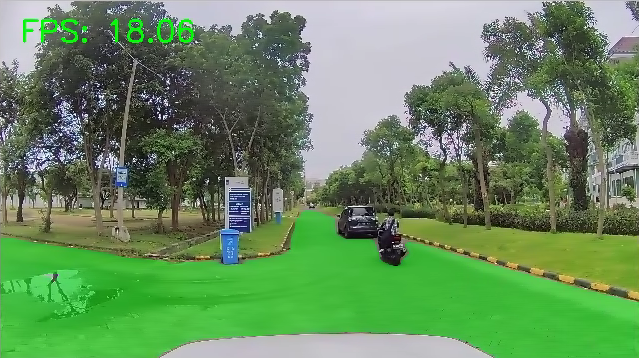
\includegraphics[width=\textwidth]{gambar/tensorrt_fps.png}
        \caption{Hasil TensorRT siang hari}
        \label{fig:tensorrt_day}
    \end{subfigure}
    \hfill
    \begin{subfigure}[b]{0.48\textwidth}
        \centering
        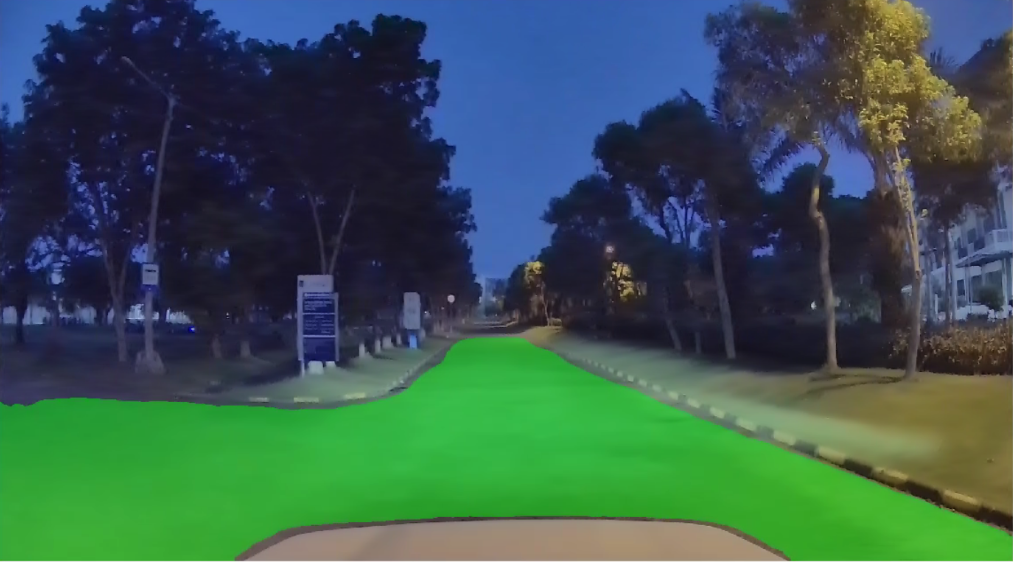
\includegraphics[width=\textwidth]{gambar/segmentasi_malam.png}
        \caption{Hasil TensorRT malam hari}
        \label{fig:tensorrt_night}
    \end{subfigure}
    \caption{Hasil segmentasi visual pada TensorRT di berbagai kondisi pencahayaan.}
    \label{fig:tensorrt_conditions}
\end{figure}

Dengan TensorRT, inferensi mencapai sekitar 18 FPS (rentang 15--19 FPS) seperti yang ditampilkan pada Gambar~\ref{fig:tensorrt_fps}, yang sudah memadai untuk navigasi \emph{real-time} pada kecepatan rendah ($\pm$8 km/jam).
Model Pytorch hanya mencapai sekitar 2 FPS sehingga tidak layak untuk aplikasi navigasi karena akan menyebabkan keterlambatan dalam pengambilan keputusan dan potensi risiko keselamatan.

\subsubsection{Konversi Mask ke \emph{Point Cloud}}
\label{sec:mask2points}

Untuk memverifikasi akurasi konversi masker biner hasil segmentasi ke representasi \emph{point cloud}, hasil konversi dibandingkan terhadap data LiDAR pada tampilan RViz.
Gambar~\ref{fig:rviz_lidar} menunjukkan bagian kiri berupa \emph{segmentation overlay} pada gambar tampak atas, dan bagian kanan berupa \emph{point cloud} hasil konversi yang ditampilkan bersama \emph{point cloud} LiDAR.
Kedua \emph{point cloud} selaras pada batas jalan, mengonfirmasi bahwa proyeksi BEV dari kalibrasi kamera telah menghasilkan representasi spasial yang sesuai.

\begin{figure}[H]
    \centering
    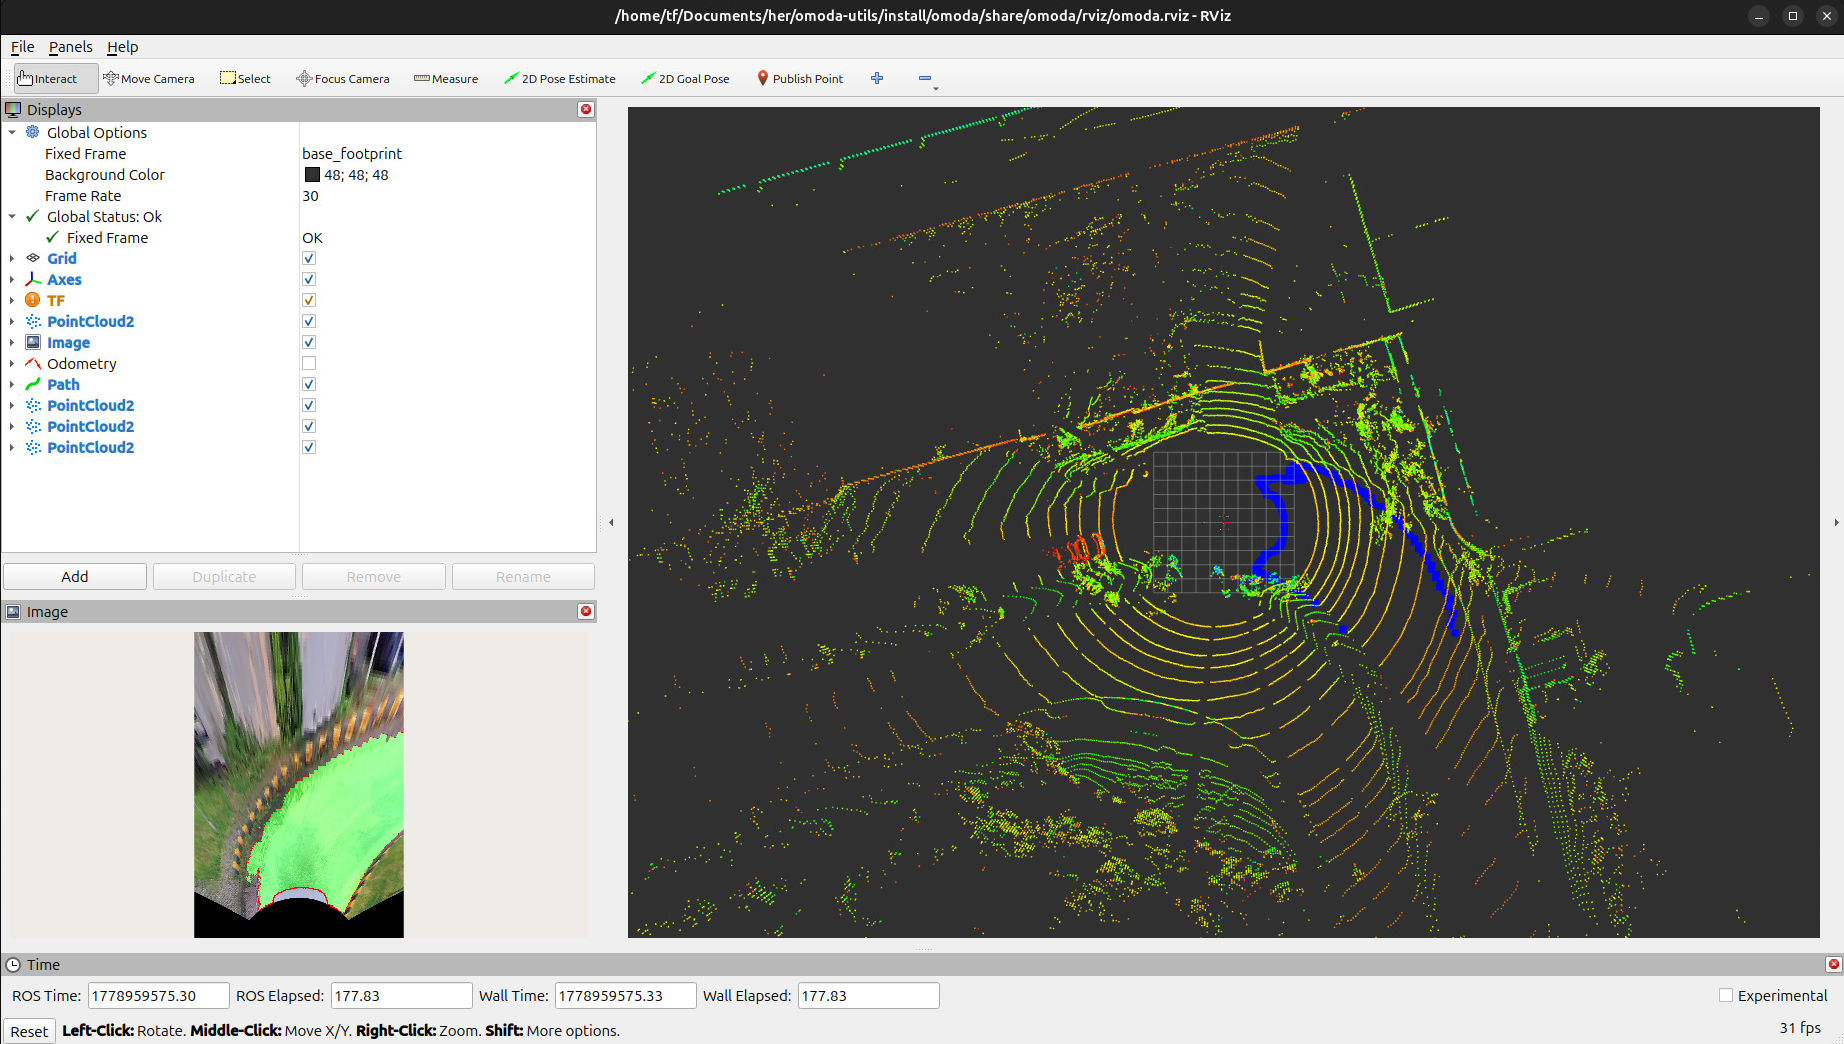
\includegraphics[width=0.95\textwidth]{gambar/rviz_pcl_camera_lidar.png}
    \caption{Verifikasi hasil konversi mask ke \emph{point cloud} terhadap LiDAR pada RViz.}
    \label{fig:rviz_lidar}
\end{figure}
